% 94-33(94쪽) — $\angle\pt{A}=60^\circ$ 인 삼각형 $\pt{ABC}$ 와 그 외접원(원문 「오른쪽 그림」). 스캔 화질이 낮아 TikZ 로 다시 그림.
% 라벨은 원문 것만: $60^\circ$ 와 꼭짓점 이름. $\seg{AB}$ 의 길이(답)가 읽히지 않게 변의 길이·반지름·눈금은 적지 않는다.
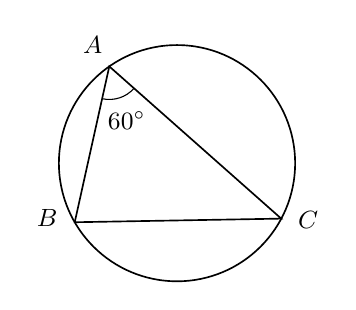
\begin{tikzpicture}[line width=0.6pt]
  \draw (0,0) circle (1.5);
  \draw (-0.860,1.229) -- (-1.299,-0.750) -- (1.324,-0.704) -- cycle;
  \draw[line width=0.4pt] (-0.951,0.819) arc (-102.5:-41.5:0.42);
  \node[font=\small] at (-0.638,0.544) {$60^\circ$};
  \node[anchor=south east, font=\small] at (-0.82,1.26) {$\pt{A}$};
  \node[anchor=east, font=\small] at (-1.39,-0.70) {$\pt{B}$};
  \node[anchor=west, font=\small] at (1.41,-0.72) {$\pt{C}$};
\end{tikzpicture}
